\section{Report Generation}

\subsection{Generating Reports}

If you should so wish it is possible to generate an XML version of the current state the application is in. This report will show you an overview of all your projects, teams, skills, people, team allocations etc so that you can get a general feel for everything in the current state of the organisation.

To reduce the size of the generated XML file not all information is explicitly added to all parts of the report. It instead is linked in other parts of the report. This prevents the duplication of data.\\
If using this report to import into another application, some preproccessing will need to be done to link data together.

\begin{figure}[H]
	\centering
	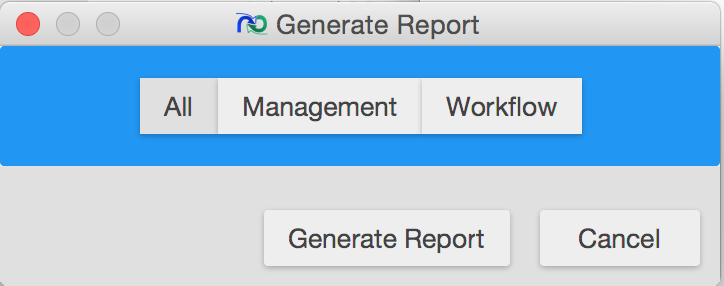
\includegraphics[width=\textwidth]{images/screenshots/report1.PNG}
	\caption{Report Generation}
	\label{fig:generate_report_all}
\end{figure}

In order to generate a report all you need to do is click on File-\textgreater Generate Report. This will open a  Report Generation Dialog which defaults to All. On this setting a complete report will be generated. Clicking generate report will bring up a save dialog asking you where you would like to save the report to. Once you have selected a location the report will be saved.

\subsection{Generating Workflow Reports}

\begin{figure}[H]
	\centering
	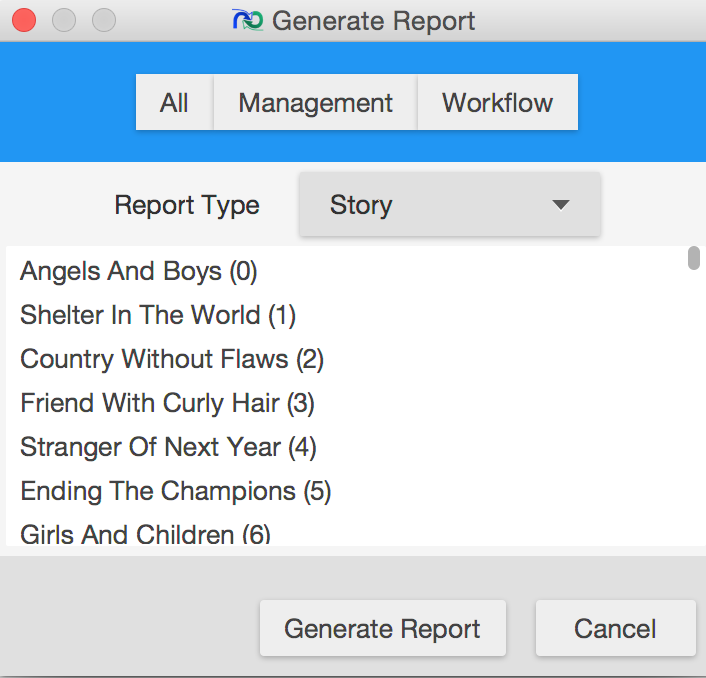
\includegraphics[width=\textwidth]{images/screenshots/report3.PNG}
	\caption{Workflow Report Generation}
	\label{fig:generate_report_workflow}
\end{figure}

A workflow report will only be able to report on things pertaining to work flow i.e. Backlogs or Stories. To generate the report, select one or more items from the list. This can be achieved by holding the CTRL key. When you are ready to generate the report.

\subsection{Generating Management Reports}

\begin{figure}[H]
	\centering
	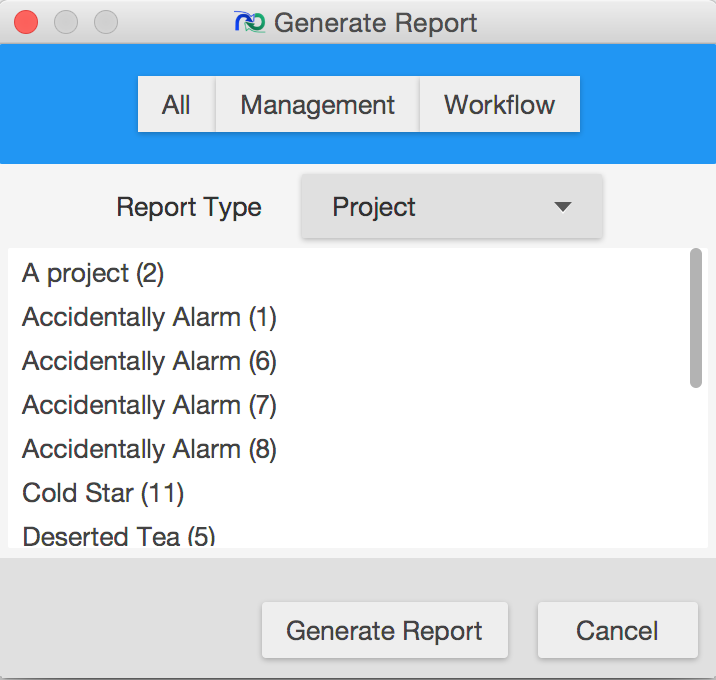
\includegraphics[width=\textwidth]{images/screenshots/report2.PNG}
	\caption{Management Report Generation}
	\label{fig:generate_report_management}
\end{figure}

A management can contain projects, teams or people. Generating a management report is similar to a workflow report. First select a type then one of more items from the list. When you are ready click generate.